\documentclass[../Homework]{subfiles}

\begin{document}
	\section{Chi-Square Tests for Goodness of Fit}
		\paragraph{1. Aw, nuts!}
			\begin{enumerate}[a.]
				\item
					\begin{align*}
						H_0&: \text{The true distribution of mixed nuts is just as the company claims.} \\
						H_a&: \text{The true distribution of mixed nuts differs from what the company claims.}
					\end{align*}
				\item
					\begin{align*}
						\text{Cashew} &= 0.52(150) = 78 = 78 & \text{Almond} &= 0.27(150) = 40.5 \\
						\text{Macadamia} &= 0.13(150) = 19.5 & \text{Brazil} &= 0.08(150) = 12
					\end{align*}
			\end{enumerate}
				\[\chi^2 = \sum\left[\mathrm{\frac{(observed - expected)^2}{expected}}\right] \approx 6.599\]
		\paragraph{3. $P$-values}
			\begin{enumerate}
				\item
					\begin{align*}
						0.05 < \pval &< 0.1 \\
						\pval &= \chiCDF{19.03}{\infty}{11} \approx 0.061
					\end{align*}
				\item
					\begin{align*}
						\pval &< 0.0005 \\
						\pval &= \chiCDF{19.03}{\infty}{3} \approx 2.695 \times 10^{-4}
					\end{align*}
			\end{enumerate}
		\paragraph{5. Aw, nuts!}
			\begin{enumerate}[a.]
				\item
					There are over 5 counts expected in each category, so the Large Counts condition is met.
					\[\df = \text{categories} - 1 = 4 - 1 = 3\]
				\item
					\begin{align*}
						0.05 < \pval &< 0.1 \\
						\pval &= \chiCDF{\chi^2 \approx 6.599}{\infty}{n - 1 = 4 - 1 = 3} \approx 0.086
					\end{align*}
				\item
					Over many trials, there is an 8.6\% probability of receiving a difference at at least as great as that observed from the claimed proportions.
				\item
					As the $\pval$ of about 8.6\% is greater than the significance level $\alpha = 0.05$, the null hypothesis cannot be rejected. The data does not provide convincing evidence that the true proportions of deluxe mixed nuts significantly differ from those claimed.
			\end{enumerate}
		\paragraph{9. Munching Froot Loops}
			\begin{align*}
				H_0&: \text{The proportions of Froot Loop colors are those claimed by Kellogg's.} \\
				H_a&: \text{The proportions of Froot Loop colors are not those claimed by Kellogg's.}
			\end{align*}
			The sample was random, so the Randomness condition is met. \\
			There are over 1200 Froot Loops, so the sample size of 120 is less than 10\% of the population size. \\
			As the probabilities are equal, the expected counts of each color is equal, being $120/6 = 20$. \\
			As the expected counts of all categories is 20, which is greater than 5, the Large Counts condition is met. \\
			\begin{align*}
				\chi^2 &= \sum\left[\mathrm{\frac{(observed - expected)^2}{expected}}\right] = 7.9 \\
				\df &= \text{categories} - 1 = 6 - 1 = 5 \\
				\pval &= \chiCDF{7.9}{\infty}{5} \approx 0.162
			\end{align*}
			As the $\pval$ of about 0.162 is greater than the significance level of $\alpha = 0.05$, the null hypothesis cannot be rejected. The data does not provide convincing evidence that the true proportions of Froot Loops colors differs from those claimed by Kellogg's.
		\paragraph{13. Birds in the tress}
			\begin{enumerate}[a.]
				\item
					\begin{align*}
						H_0&: \text{The red-breasted nuthatches have no preference regarding trees.} \\
						H_a&: \text{The red-breasted nuthatches have some preference regarding trees.}
					\end{align*}
					The sample was random, so the Randomness condition is met. \\
					The sample size of 156 is likely less than 10\% of the number of red-breasted nuthatches in the forest, so the 10\% condition is met, justifying independence. \\
					\begin{align*}
						\text{Douglas firs} &= (0.54)(312) = 84.24 & \text{ponderosa pines} &= (0.4)(156) = 62.4 \\
						\text{other} &= (0.06)(156) = 9.36
					\end{align*}
					The expected counts of each category are greater than 5, so the Large Counts condition is met. \\
					\begin{align*}
						\chi^2 &= \sum\left[\mathrm{\frac{(observed - expected)^2}{expected}}\right] \approx 7.418 \\
						\df &= \text{categories} - 1 = 3 - 1 = 2 \\
						\pval &= \chiCDF{\chi^2 \approx 7.418}{\infty}{2} \approx 0.024 
					\end{align*} \\
					As the $\pval$ of about 0.024 is less than the significance level $\alpha = 0.05$, the null hypothesis can be rejected. The data provides convincing evidence that red-breasted nuthatches have some preference regarding trees.
				\item
					\[\begin{array}{|c|c|c|c|}\hline
						\text{tree} & \text{observed} & \text{expected} & \mathrm{observed - expected} \\\hline
						\text{Douglas firs} & 70 & 84.24 & -14.24 \\\hline
						\text{ponderosa pines} & 79 & 62.4  & 16.6 \\\hline
						\text{other} & 7 & 9.36 & -2.36 \\\hline
					\end{array}\]
					The greatest (and only) positive difference between the observed and expected counts indicates that red-breasted nuthatches prefer ponderosa pines. The greatest negative difference indicates that they are most averse to Douglas firs.
			\end{enumerate}
		\paragraph{15. Mendel and the peas}
			\begin{enumerate}[a.]
				\item
					\begin{align*}
						H_0&: \text{The actual proportions of smooth and wrinkled peas are 0.75 and 0.25 respectively.} \\
						H_a&: \text{The actual proportions of smooth and wrinkled peas are not \(0.75\) and \(0.25\) respectively}
					\end{align*}
					\[\begin{array}{|c|c|c|}\hline
						\text{pea} & \text{observed} & \text{expected} \\\hline
						\text{smooth} & 423 & 0.75(423 + 133) = 417 \\\hline
						\text{wrinkled} & 133 & 0.25(423 + 133) = 139 \\\hline
					\end{array}\]
					\begin{align*}
						\chi^2 &= \sum\left[\mathrm{\frac{(observed - expected)^2}{expected}}\right] \approx 0.345 \\
						\df &= \text{categories} - 1 = 2 - 1 = 1 \\
						\pval &= \tCDF{\chi^2 \approx 0.345}{\infty}{1} \approx 0.557
					\end{align*}
					As the $\pval$ of about 0.557 is greater than the significance level $\alpha = 0.05$, the null hypothesis cannot be rejected. The data does not provide convincing evidence that the true proportions of smooth and wrinkled peas are not 0.75 and 0.25 respectively.
				\item
					\begin{align*}
						\hat{p} &= \frac{423}{423 + 133} \approx 0.761 \\
						s_{\hat{p}} &= \propse{\hat{p}}{n} \approx \propse{0.761}{423 + 133} \approx 0.018 \\ 
						z &= \z{\hat{p}}{p_0}{s_{\hat{p}}} \approx \z{0.761}{0.75}{0.018} \approx 0.596 \\
						\pval &= 1 - \normalCDF{-z \approx -0.596}{z \approx 0.596}{0}{1} \approx 0.551
					\end{align*}
					As the $\pval$ of about 0.551 is greater than the significance level $\alpha = 0.05$, the null hypothesis cannot be rejected. The data does not provide convincing evidence that the true proportion smooth peas is not equal to 0.75.
			\end{enumerate}
		\paragraph{17. Is your random number generator working?}
			\begin{enumerate}[a.]
				\item
					\begin{align*}
						H_0&: \text{Each digit's proportion is 0.1.} & H_a&: \text{Not every digit's proportion is 0.1}
					\end{align*}
					The randomness condition is met, as the numbers were randomly generated. \\
					The independence condition is met, as each digit being generated was independent of the last. \\
					\[\begin{array}{|c|c|c|c|c|c|c|c|c|c|c|}\hline
						\text{digit} & 0 & 1 & 2 & 3 & 3 & 5 & 6 & 7 & 8 & 9 \\\hline
						\text{observed} & 18 & 20 & 25 & 25 & 21 & 15 & 18 & 19 & 13 & 26 \\\hline
						\text{expected} & 0.1(200) = 20 & 20 & 20 & 20 & 20 & 20 & 20 & 20 & 20 & 20 \\\hline
					\end{array}\]
					The Large Counts condition is met, as each digit is expected to be generated 20 times, which is greater than 5.
				\item
					\begin{align*}
						\chi^2 &= \sum\left[\mathrm{\frac{(observed - expected)^2}{expected}}\right] = 6.7 \\
						\df &= \text{categories} - 1 = 10 - 1 = 9 \\
						\pval &= \chiCDF{\chi^2 = 6.7}{\infty}{9} \approx 0.668
					\end{align*}
					As the $\pval$ of 0.668 is greater than the significance level $\alpha = 0.05$, the null hypothesis cannot be rejected. The data does not provide convincing evidence of the true proportions of randomly generated digits being nonuniform. \\
				\item
					The probability of a Type \Roman{1} error occurring is equal to the significance level $\alpha = 0.05$. \\
				\item
					The probability of a Type \Roman{1} error occurring is the same for every trial. \\
					The number of trials is fixed at 25. \\
					A Type \Roman{1} error can either occur or not occur, making the outcome binary. \\
					The number of Type \Roman{1} errors is therefore a binomial variable.
					\[P(X \ge 1) = 1 - P(X = 0) = 1 - \binom{25}{0}(0.05)^0(1 - 0.05)^{25 - 0} \approx 0.277\]
			\end{enumerate}
		\paragraph{19.}\ \\
			The null hypothesis should describe population proportions, making the answer \textbf{d}.
		\paragraph{20.}
			\[\chi^2 = \sum\left[\mathrm{\frac{(observed - expected)^2}{expected}}\right]\]
			The answer is therefore \textbf{a}.
		\paragraph{21.}\ \\
			A $\pval$ less than the significance level results in $H_0$ being rejected due to the data providing convincing evidence for $H_a$. The answer is therefore \textbf{c}.
		\paragraph{22.}\ \\
			The degrees of freedom for a chi-square test is determined by the number of categories, not the sample size. The answer is therefore \textbf{c}.
		\paragraph{23. Video games}
			\begin{enumerate}[a.]
				\item\
					\begin{center}
						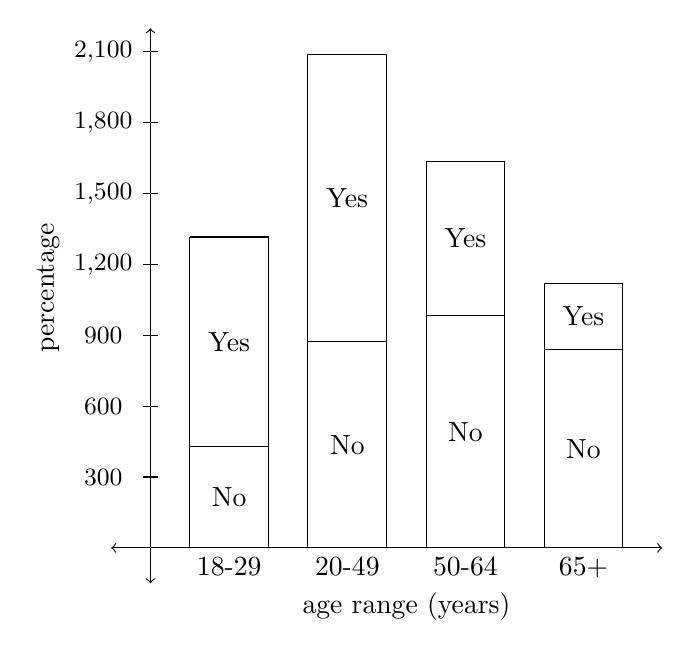
\begin{tikzpicture}[yscale = 3]
							%Axes
							%TODO Fix (standardize)
							\draw[<->] (-0.5, 0) -- (6.5, 0);
								\node[] at (6.5/2, -0.25) {age range (years)};
							\draw[<->] (0, -0.15) -- (0, 2.2);
								\node[rotate = 90] at (-1.3, 2.2/2) {percentage};
							\foreach \x in {1,...,7}
								\draw[] (-0.1, \x * 0.3) -- (0.1, \x * 0.3);
							\foreach \x in {1,...,7}
								\pgfmathparse{\x * 300} \pgfmathprintnumberto{\pgfmathresult}\fx
								\node at (-0.6, \x * 0.3) {\small \fx};
							%Columns
							 	%18-29
								\draw[] (0.5, 0) -- (0.5, 1.316);
								\draw[] (1.5, 0) -- (1.5, 1.316);
								\draw[] (0.5, 1.316) -- (1.5, 1.316);
								\draw[] (0.5, 0.429) -- (1.5, 0.429);
								\node[below] at (1, 0) {18-29};
								\node[] at (1, 0.429/2) {No};
								\node[] at (1, 0.887/2 + 0.429) {Yes};
								%30-49
								\draw[] (2, 0) -- (2, 2.089);
								\draw[] (3, 0) -- (3, 2.089);
								\draw[] (2, 2.089) -- (3, 2.089);
								\draw[] (2, 0.872) -- (3, 0.872);
								\node[below] at (2.5, 0) {20-49};
								\node[] at (2.5, 0.872/2) {No};
								\node[] at (2.5, 1.217/2 + 0.872) {Yes};
								%60-64
								\draw[] (3.5, 0) -- (3.5, 1.635);
								\draw[] (4.5, 0) -- (4.5, 1.635);
								\draw[] (3.5, 1.635) -- (4.5, 1.635);
								\draw[] (3.5, 0.985) -- (4.5, 0.985);
								\node[below] at (4, 0) {50-64};
								\node[] at (4, 0.985/2) {No};
								\node[] at (4, 0.65/2 + 0.985) {Yes};
								%65+
								\draw[] (5, 0) -- (5, 1.119);
								\draw[] (6, 0) -- (6, 1.119);
								\draw[] (5, 1.119) -- (6, 1.119);
								\draw[] (5, 0.84) -- (6, 0.84);
								\node[below] at (5.5, 0) {65+};
								\node[] at (5.5, 0.84/2) {No};
								\node[] at (5.5, 0.279/2 + 0.84) {Yes};
						\end{tikzpicture}
					\end{center}
				\item
					The lower the age, the higher the proportion of people that play video games.
			\end{enumerate}
	\section{Inference for Two-Way Tables}
		\paragraph{27. The color of candy}\ \\
			Those that took a colored survey showed a strong preference for the candy of the same color while those in the control group slightly preferred the blue candy.
		\paragraph{29. More candy}
			\begin{enumerate}[a.]
				\item		
					\begin{align*}
						H_0&: \text{The distributions of candy colors remains the same regardless of the survey.} \\
						H_a&: \text{The distributions of candy colors is affected by the survey.}
					\end{align*}
				\item
					\[\begin{tabular}{|c|c|c|}\hline
						& Red & Blue \\\hline
						Red & $\frac{20(26)}{60} = 8.\overline{3}$ & $\frac{20(26)}{60} = 8.\overline{3}$ \\\hline
						Blue & $\frac{20(34)}{60} = 11.\overline{3}$ & $\frac{20(34)}{60} = 11.\overline{3}$ \\\hline
					\end{tabular}\]
				\item
					\[\chi^2 = \sum\left[\mathrm{\frac{(observed - expected)^2}{expected}}\right] \approx 6.652\]
			\end{enumerate}			
		\paragraph{31. Last candy}
			\begin{enumerate}[a.]
				\item
					The Randomness condition is met, as the assignment was random. \\
					The independence condition is met, as this is an experiment. \\
					The Large Counts condition is met, as all expected values are greater than 5.
				\item
					\begin{align*}
						0.005 < \pval &< 0.01 \\
						\pval &= \tCDF{\chi^2 \approx 6.652}{\infty}{(2 - 1)(3 - 1) = 2} \approx 0.036
					\end{align*}
				\item
					If the survey has no affect on preferences, the probability of receiving data that differ from the expected values at least as much as those observed is about 3.6\%.
				\item
					As the $\pval$ of about 0.036 is greater than the significance level $\alpha = 0.01$, the null hypothesis cannot be rejected. The data does not provide convincing evidence that the survey affects the preferences for candy color.
			\end{enumerate}
		\paragraph{33. Sorry, no chi-square}\ \\
			The counts of the travelers from each category is not known, just the relative frequencies of each category.
		\paragraph{34. Going nuts}\ \\
			The data describes means rather than counts (proportions).
		\paragraph{35. Gummy bears}
			\begin{align*}
				H_0&: \text{The distributions of colors is the same for name and store-brand gummy bears} \\
				H_a&: \text{The distributions of colors differs for name and store-brand gummy bears}
			\end{align*}
			The randomness condition is met, as the samples were random. \\
			The independence condition is met, as there are over 6 bags is far less than 10\% of the number of bags of name or store-brand gummy bears. \\
			\[\begin{tabular}{|c|c|c|}\hline
				& Name & Store \\\hline
				Red & 130.83 & 218.17 \\\hline
				Green & 58.86 & 98.15 \\\hline
				Yellow & 50.61 & 84.39 \\\hline
				Orange & 77.97 & 130.03 \\\hline
				White & 54.742 & 91.268 \\\hline
			\end{tabular}\]
			Every expected count exceeds 5, so the Large Counts condition is met.
			\begin{align*}
				\chi^2 &= \sum\left[\mathrm{\frac{(observed - expected)^2}{expected}}\right] \approx 1.815 \\
				\df &= (2 - 1)(5 - 1) = 4 \\
				\pval &= \chiCDF{\chi^2 \approx 1.815}{\infty}{4} \approx 0.77
			\end{align*}
			As the $\pval$ of about 0.77 is greater than the significance level $\alpha = 0.05$, the null hypothesis cannot be rejected. The data does not provide convincing evidence of a difference existing between the true distributions of gummy bear colors for name and store brands.
		\paragraph{37. How to quit smoking}
			\begin{enumerate}[a.]
				\item
					\[\begin{tabular}{|c|c|c|c|c|c|}\hline
						& Nicotine patch & Drug & Patch plus drug & Placebo & Total \\\hline
						Successes & 40 & 74 & 87 & 25 & 226  \\\hline
						Failures & 204 & 170 & 158 & 135 & 667 \\\hline
						Total & 244 & 244 & 245 & 160 & 893 \\\hline
					\end{tabular}\]
				\item
					\begin{align*}
						H_0&: \text{The proportions of successes and failures is the same across all treatments.} \\
						H_a&: \text{The proportions of successes and failures is not the same across all treatments.}
					\end{align*}
					The randomness condition is met, as the assignment was random. \\
					The independence condition is met, as this is an experiment. \\
					\[\begin{tabular}{|c|c|c|c|c|}\hline
						& Nicotine patch & Drug & Patch plus drug & Placebo \\\hline
						Successes & 61.75 & 61.75 & 62 & 40.49 \\\hline
						Failures & 182.25 & 182.25 & 183 & 119.51 \\\hline
					\end{tabular}\]
					Every expected count is greater than 5, so the Large Counts condition is met.
					\begin{align*}
						\chi^2 &= \sum\left[\mathrm{\frac{(observed - expected)^2}{expected}}\right] \approx 34.937 \\
						\df &= (4 - 1)(2 - 1) = 3 \\
						\pval &= \chiCDF{\chi^2 \approx 34.937}{\infty}{3} \approx 1.256 \times 10^{-7}
					\end{align*}
					As the $\pval$ of about $1.256 \times 10^{-7}$ is less than the significance level $\alpha = 0.05$, the null hypothesis can be rejected. The data provides convincing evidence that different treatments result in a different distribution of successes and failures.
			\end{enumerate}
		\paragraph{39. How to quit smoking}\ \\
			The treatment with the largest positive difference between its actual and expected values is the combination of the patch and drug, suggesting that is is the most effective. The one with the largest negative difference, on the other hand, is the nicotine patch, indicating that it is the least effective treatment.
		\paragraph{41. Relaxing in the sauna}
			\begin{enumerate}[a.]
				\item
					\begin{align*}
						H_0&: \text{The distribution of suffering from SCD is independent of weekly sauna frequency.} \\
						H_a&: \text{Weekly sauna frequency affects the distribution of suffering from SCD.}
					\end{align*}
				\item
					\[\begin{tabular}{|c|c|c|c|}\hline
						& $<1$ & 2--3 & $>4$ \\\hline
						Yes & 49.33 & 124.18 & 17.5 \\\hline
						No & 551.67 & 1388.8 & 184.5 \\\hline
					\end{tabular}\]
				\item
					\begin{align*}
						\chi^2 &= \sum\left[\mathrm{\frac{(observed - expected)^2}{expected}}\right] \approx 6.032 \\
						\df &= (3 - 1)(2 - 1) = 2 \\
						\pval &= \chiCDF{\chi^2 \approx 6.032}{\infty}{2} \approx 0.049
					\end{align*}
				\item
					As the $\pval$ of about 0.049 is less than the significance level $\alpha = 0.05$, the null hypothesis can be rejected. The data provides convincing evidence that going to the sauna affects the distribution of SCD suffering.
			\end{enumerate}
		\paragraph{43. Finger length}
			\begin{align*}
				H_0&: \text{There is no association between gender and relative finger length in this population.} \\
				H_a&: \text{There is an association between gender and relative finger length in this population.}
			\end{align*}
			As an association between categorical variables is being tested, a chi-square test for independence should be performed. \\
			The sample was random, so the randomness condition is met. \\
			There 10\% condition is met, as there are far over 2270 and 2230 female and male high school students respectively.
			\[\begin{tabular}{|c|c|c|}\hline
				& Female & Male \\\hline
				Index longer & 77.97 & 80.03 \\\hline
				Same length & 42.439 & 43.561 \\\hline
				Ring longer & 106.591 & 109.409 \\\hline
			\end{tabular}\]
			As all expected counts are greater than 5, the Large Counts condition is met.
			\begin{align*}
				\chi^2 &= \sum\left[\mathrm{\frac{(observed - expected)^2}{expected}}\right] \approx 2.065 \\
				\df &= (2 - 1)(3 - 1) = 2 \\
				\pval &= \chiCDF{\chi^2 \approx 2.065}{\infty}{2} \approx 0.356
			\end{align*}
			As the $\pval$ of about 0.356 is greater than the significance level $\alpha = 0.1$, the null hypothesis cannot be rejected. The data does not provide convincing evidence of an association existing between gender and relative finger length in this population.
		\paragraph{47. Which test?}
			\begin{enumerate}[a.]
				\item
					The data came from two random samples, so a chi-square test for homogeneity should be performed.
				\item
					The data came from a single random sample and an association between two categorical variables is being assessed, so a chi-square test for independence should be performed.
			\end{enumerate}
		\paragraph{53. Treating ulcers}
			\begin{enumerate}[a.]
				\item
					$H_0:$ There is no difference between the improvement rates for patients given gastric-freezing and placebo treatments. \\
					$H_a:$ There is a difference between the improvement rates for patients given the gastric-freezing and placebo treatments.
				\item
					As the $\pval$ of 0.57 is greater than the significance level $\alpha = 0.05$, the null hypothesis cannot be rejected. The data does not provide convincing evidence of a difference between the improvement rates for patients given the gastric-freezing and placebo treatments.
				\item
					The $\pval$s of both tests are equal.
			\end{enumerate}
	\section{Inference for Slopes}
		\paragraph{65. Predicting height}
			\begin{enumerate}[a.]
				\item
					\[\mu_y = 105 + 4.2(15) = 168\,\text{cm}\]
				\item
					\begin{align*}
						z &= \z{y}{\mu_y}{\sigma_y} = \z{180}{168}{7} \approx  1.714 \\
						P(Z > z) &= \normalCDF{z \approx 1.714}{\infty}{0}{1} \approx 0.043 = 4.3\%
					\end{align*}
				\item
					The slope of the sample regression line would likely not be exactly 4.2, as a single sample is unlikely to perfectly represent the population.
			\end{enumerate}
		\paragraph{66. Predicting high temperatures}
			\begin{enumerate}[a.]
				\item
					\[\mu_y = 16.6 + 1.02(40) = 57.4\,^\circ\mathrm{F}\]
				\item
					\begin{align*}
						z &= \z{y}{\mu_y}{\sigma_y} = \z{70}{57.4}{6.64} \approx 1.898 \\
						P(Z > z) &= \normalCDF{z \approx 1.898}{\infty}{0}{1} \approx 0.029 = 2.9\%
					\end{align*}
				\item
					A random sample, especially one of a size as small as 10, is unlikely to perfectly represent the population, so the slope would likely differ.
			\end{enumerate}
		\paragraph{67. Oil and residuals}\ \\
			The residual plot shows that the standard deviation of the residuals increases with the explanatory variable, meaning that the standard deviation of the response variable is dependent on the explanatory variable, preventing inference.
		\paragraph{68. SAT Math scores}\ \\
			A nonrandom pattern is displayed on the residual plot, indicating that the explanatory and response variables are nonlinearly related, preventing inference regarding the regression.
		\paragraph{69. Beer and BAC}\ \\
			The residual plot displays a random pattern, indicating that the response and explanatory variables follow a linear relationship. \\
			The independence condition is met by the 10\% conditions, as there are far more 160 adults aged over 21, making the sample size of 16 less than a tenth of the population size. \\
			The distribution of the explanatory variable lacks strong skew or outliers, meaning that the Normality condition is met. \\
			The variability of the residuals is about the same for every value of the explanatory variable. \\
			The randomness condition is met, as the assignment was random.
		\paragraph{71. Beer and BAC}
			\begin{enumerate}[a.]
				\item
					The estimate for $\alpha$ is the constant coefficient, which is $-0.012701$. When no beers are drunk, the BAC is estimated to be $-0.012701$.
				\item
					The estimate for $\beta$ is the beers coefficient, which is 0.017964. An increase in beers drank of 1 results in BAC increasing by 0.017964.
				\item
					The estimate for $\sigma_y$ is $s$, which is 0.0204. The actual BAC varies by an average of 0.0204 from the amount predicted by the least-square regression line.
				\item
					The standard error of the slope $s_b$ is 0.0024. If the random assignment were to be repeated many times, the sample slope would vary from the true slope by an average of 0.0024.
			\end{enumerate}
		\paragraph{73. Beer and BAC}
			\begin{enumerate}[a.]
				\item
					\begin{align*}
						\df &= n - 2 = 16 - 2 = 14 \\
						t^* &= \left|\invT{\tarea{0.99} = 0.005}{15}\right| \approx 2.977 \\
						\ME &= t^*s_b \approx 2.977 \times 0.0024 \approx 0.007 \\
						\cint &= b \pm \ME \approx 0.018 \pm 0.007 = (0.001, 0.025)
					\end{align*}
				\item
					It can be said with 99\% confidence that the true slope $\beta$ of the population least-squares regression line relating BAC to beers drank is within the interval $(0.001, 0.025)$.
				\item
					Over many samples, 99\% of the confidence intervals constructed at the 99\% confidence level will contain the true population slope.
				\item
					As 0 is not contained within the confidence interval, there is convincing evidence of a linear association existing between number of beers drank and BAC.
			\end{enumerate}
		\paragraph{75. Less mess?}
			\begin{align*}
				Y &= \text{amount of soda expelled (mL)} \\
				X &= \text{time spent tapping} \\
				\beta &= \text{slope of the population regression line relating Y to X}
			\end{align*}
			The residual plot shows a random pattern, indicating a linear relationship between time spent tapping and the amount of soda expelled. \\
			The independence condition is met, as this is an experiment. \\
			The Normality condition is met, as the distribution of the residuals lacks any strong skew or outliers. \\
			The variability and therefore the standard deviation of the residuals appears to be constant regardless of the time spent tapping. \\
			The assignment was random.
			\begin{align*}
				\df &= n - 2 = 40 - 2 = 38 \\
				t^* &= \left|\invT{\tarea{0.95} = 0.025}{38}\right| \approx 2.024 \\
				\ME &= t^*s_b \approx 2.024 \times 0.177 \approx 0.237 \\
				\cint &= b \pm \ME \approx -2.635 \pm 0.237 \approx (-2.872, 2.398)
			\end{align*}
			It can be said with 95\% confidence that the slope of the population regression line relating the amount of soda expelled and time spent tapping is contained within the interval $(-2.872, 2.398)$.
		\paragraph{77. Beavers and beetles}
			\begin{enumerate}[a.]
				\item
					\begin{align*}
						Y &= \text{clusters of beetle larvae} \\
						X &= \text{trees cut by beavers} \\
						\beta &= \text{slope of the population regression line relating $Y$ to $X$}
					\end{align*}
					\begin{align*}
						\df &= n - 2 = 23 - 2 = 21 \\
						t^* &= \left|\invT{\tarea{C} = \tarea{0.99} = 0.005}{21}\right| \approx 2.831 \\
						\ME &= t^*s_b \approx 2.831 \times 1.136 \approx 3.216 \\
						\cint &= b \pm \ME \approx 11.894 \pm 3.216 \approx (8.678, 15.11)
					\end{align*}
					It can be said with 99\% confidence that the true slope of the population regression line relating the number of clusters of beetle larvae and that of trees cut by beavers is contained within the interval $(8.678, 15.11)$.
				\item
					The width of the confidence interval, double the margin of error, can be reduced by either increasing the sample size, increasing $\df$ and therefore reducing $t^*$ in addition to reducing $s_b$, or by reducing the confidence level, reducing $t^*$. The former would be more expensive and time consuming while the latter would result in a confidence interval that is less likely to contain the true slope.
			\end{enumerate}
		\paragraph{79. Weeds among the corn}
			\begin{align*}
				Y &= \text{yield} & X &= \text{weeds per meter} & \beta &= \text{slope of regression line relating $Y$ to $X$}
			\end{align*}
			\begin{align*}
				H_0&: \beta = 0 & H_a&: \beta < 0
			\end{align*}
			The residual plot shows a random pattern, indicating a linear relationship between $Y$ and $X$. \\
			The data was collected in an experiment, so each observation is independent. \\
			The residual plot lacks strong skew or outliers, so Normality is justified. \\
			The spread of the residuals looks to be fairly constant regardless of the number of weeds per meter, indicating the standard deviation of $Y$ is as well. \\
			The assignment was random.
			\begin{align*}
				t &= \z{b}{\beta_0}{s_b} \approx \z{-1.099}{0}{0.571} \approx -1.923 \\
				\df &= n - 2 = 16 - 2 = 14 \\
				\pval &= \tCDF{-\infty}{t \approx -1.923}{14} \approx 0.038
			\end{align*}
			As the $\pval$ of about 0.038 is less than the significance level $\alpha = 0.05$, the null hypothesis can be rejected. The data provides convincing evidence that the population regression line relating yield to weeds per meter has a negative slope.
		\paragraph{83 Turn up the volume?}
			\begin{enumerate}[a.]
				\item
					\[\beta = \text{Slope of regression line relating Y to X}\]
					\begin{align*}
						H_0&: \beta = 0 & H_a&: \beta < 0
					\end{align*}
					\begin{align*}
						t &= \z{b}{\beta_0}{s_b} = \z{-0.0483}{0}{0.0116} \approx -4.164 \\
						\df &= n - 2 = 30 - 2 = 28 \\
						\pval &= \tCDF{-\infty}{t \approx -4.164}{28} \approx 1.351 \times 10^{-4}
					\end{align*}
					As the $\pval$ of about $1.351 \times 10^{-4}$ is less than the significance level $\alpha = 0.05$, the null hypothesis can be rejected. The data provides convincing evidence that the volume of music and the number of correct test questions are negatively associated.
				\item
					Over many trials of size 30 of the same experiment, assuming $H_0$ to be true, the probability of receiving results that support the null hypothesis at least as strongly as those observed here is about $1.351 \times 10^{-4}$.
			\end{enumerate}
		\paragraph{85. Stats teachers' cars}
			\begin{enumerate}[a.]
				\item
					\begin{align*}
						\df &= n - 2 = 21 - 2 = 19 \\
						t^* &= \left|\invT{\tarea{c} = \tarea{0.95} = 0.025}{19}\right| \approx 2.093 \\
						\ME &= t^*s_b \approx 2.094 \times 1249 \approx 2614.187 \\
						\cint &= b \pm \ME \approx 11630.6 \pm 2614.187 \approx (9016.413, 14244.787)
					\end{align*}
				\item
					The test is attempting to determine whether a specific subset of a population differs significantly from the population at large regarding a rate relating a period of time to a quantitative value, so a 2-sided test about a population slope should be performed.
				\item
					\begin{align*}
						t &= \z{b}{\beta_0}{s_b} = \z{11630.6}{15000}{1249} \approx -2.698 \\
						\pval &= \tCDF{-\infty}{t \approx -2.698}{19} \approx 0.00713
					\end{align*}
					As the $\pval$ of about 0.00713 is less than the significance level $\alpha = 0.05$, the null hypothesis can be rejected. The data provides convincing evidence that the true average number of miles put on their primary vehicle per year for an AP\textsuperscript{\textregistered} Statistics teacher differs from that of an average person (15000).
				\item
					The confidence interval and significance tests led to the same conclusions, as 15000 was not contained within the interval.
			\end{enumerate}
		\paragraph{87.}
			\[\hat{y} = 91.9766 + 3.0867x\]
			The answer is therefore \textbf{c}.
		\paragraph{88.}\ \\
		The slope of the \emph{population} regression line represents the average change in the response variable for a change of 1 in the explanatory variable. The answer is therefore \textbf{c}.
		\paragraph{89.}
			\begin{align*}
				H_0&: \beta = 0 & H_a&: \beta > 0
			\end{align*}
			The answer is therefore \textbf{a}.
		\paragraph{91.}\ \\
			0.4117 is the standard error of the sample slope, so the answer is therefore \textbf{e}.
		\paragraph{92.}\ \\
			\begin{align*}
				\df &= n - 2 = 25 - 2 = 23 \\
				t^* &= \left|\invT{\tarea{C} = \tarea{0.95} = 0.025}{23}\right| \approx 2.069 \\
				\ME &= t^*s_b \approx 2.069 \times 0.4117 \approx 0.8517 \\
				\cint &= b \pm \ME \approx 3.8076 \pm 0.8517
			\end{align*}
			The answer is therefore \textbf{b}.
\end{document}